\documentclass{article}
\usepackage{amsmath}
\usepackage{caption}
\usepackage{multirow}
\usepackage{wrapfig}
\usepackage[T2A]{fontenc}
\usepackage[english,russian]{babel}
\usepackage{graphicx}
\usepackage{subcaption}
\usepackage[a4paper,top=2cm,bottom=2cm,left=1.5cm,right=1.5cm,marginparwidth=1.75cm]{geometry}
\usepackage{indentfirst}
\usepackage{physics}
\usepackage{mathtools}
\usepackage{extarrows}
\usepackage{nicefrac}

\usepackage[colorlinks=true, allcolors=blue]{hyperref}

\newcommand{\x}{\text}
\newcommand{\ii}{\textit}
\newcommand{\bb}{\textbf}
\newcommand*\textfrac[2]{
  \frac{\text{#1}}{\text{#2}}
}

\date{}
\author{}
\title{Лaбораторная работа 2.1.3 \\ Определение $C_P/C_V$ по скорости звука в газе}

\begin{document}
\maketitle

\section*{Введение}
\textbf{Цель работы:}  \begin{enumerate}
	\item измерение частоты колебаний и длины волны при резонансе звуковых колебаний в газе, заполняющем трубу;
	\item определение показателя адиабаты с помощью уравнения состояния идеального газа.
\end{enumerate}

\textbf{В работе используются:} звуковой генератор ГЗ; электронный осциллограф ЭО; микрофон; телефон; раздвижная труба; теплоизолированная труба, обогреваемая водой из термостата; баллон со сжатым углекислым газом; газгольдер.

\section*{Теоретические сведения}

Скорость распространения звуковой волны в газах зависит от показателя адиабаты $ \gamma $. На измерении скорости звука основан один из наиболее точных методов определения показателя адиабаты.

Скорость звука в газах определяется формулой:

\begin{equation}\label{velocity}
	c=\sqrt{\gamma\frac{RT}{\mu}}.
\end{equation}
где $ R $ -- газовая постоянная, $ T $ -- температура газа, а $ \mu $ -- его молярная масса. Преобразуя эту формулу, найдем
\begin{equation}\label{gamma}
	\boxed{\gamma = \frac{\mu}{RT}c^2}.
\end{equation}

Таким образом, для определения показателя адиабаты достаточно измерить температуру газа и скорость распространения звука (молярная масса газа предполагается известной).

Звуковая волна, распространяющаяся вдоль трубы, испытывает многократные отражения от торцов. Звуковые колебания в трубе являются наложением всех отраженных волн и очень сложны. Картина упрощается, если длина трубы $ L $ равна целому числу полуволн, то есть когда \[ L=n\lambda/2, \] где $ \lambda $ -- длина волны звука в трубе, а $ n $ -- любое целое число. Если это условие выполнено, то волна, отраженная от торца трубы, вернувшаяся к ее началу и вновь отраженная, совпадает по фазе с падающей. Совпадающие по фазе волны усиливают друг друга. Амплитуда звуковых колебаний при этом резко возрастает -- наступает резонанс.

При звуковых колебаниях слои газа, прилегающие к торцам трубы, не испытывают смещения. Узлы смещения повторяются по всей длине трубы через $ \lambda/2 $. Между узлами находятся максимумы смещения.

Скорость звука c связана с его частотой $ f $ и длиной волны $ \lambda $ соотношением

\begin{equation}\label{lambda_f}
	c=\lambda f.
\end{equation}

Подбор условий, при которых возникает резонанс, можно производить двояко:
\begin{enumerate}
	\item При неизменной частоте $ f $ звукового генератора (а следовательно, и неизменной длине звуковой волны $ \lambda $) можно изменять длину трубы $ L $. Для этого применяется раздвижная труба. Длина раздвижной трубы постепенно увеличивается, и наблюдается ряд последовательных резонансов. Возникновение резонанса легко наблюдать на осциллографе по резкому увеличению амплитуды колебаний. Для последовательных резонансов имеем \begin{equation}\label{first}
		      L_n=n\frac{\lambda}{2}, \quad L_{n+1}=(n+1)\frac{\lambda}{2}, \quad \dots, \quad L_{n+k} = n\frac{\lambda}{2}+k\frac{\lambda}{2},
	      \end{equation} т. е. $ \lambda/2 $ равно угловому коэффициенту графика, изображающего зависимость длины трубы $ L $ от номера резонанса $ k $. Скорость звука находится по формуле \eqref{lambda_f}.
	\item При постоянной длине трубы можно изменять частоту звуковых колебаний. В этом случае следует плавно изменять частоту $ f $ звукового генератора, а следовательно, и длину звуковой волны $ \lambda $. Для последовательных резонансов получим
	      \begin{equation}\label{4}
		      L=\frac{\lambda_1}{2}n=\frac{\lambda_2}{2}(n+1)=\dots=\frac{\lambda_{k+1}}{2}(n+k).
	      \end{equation}

	      Из \eqref{lambda_f} и \eqref{4} имеем:
	      \[ f_1=\frac{c}{\lambda_1}=\frac{c}{2L}n, \quad f_2=\frac{c}{\lambda_2}=\frac{c}{2L}(n+1)=f_1+\frac{c}{2L},\quad \dots, \]
	      \begin{equation}\label{5}
		      f_{k+1}=\frac{c}{\lambda_{k+1}}=\frac{c}{2L}(n+k)=f_1+\frac{c}{2L}k.
	      \end{equation}
	      Скорость звука, деленная на $ 2L $, определяется, таким образом, по угловому коэффициенту графика зависимости частоты от номера резонанса.
\end{enumerate}

\section*{Экспериментальная установка}

Соответственно двум методам измерения скорости звука в работе имеются две установки. В обеих установках звуковые колебания в трубе возбуждаются телефоном Т и улавливаются микрофоном М. Мембрана телефона приводится в движение переменным током звуковой частоты; в качестве источника переменной ЭДС используется звуковой генератор ГЗ. Возникающий в микрофоне сигнал наблюдается на осциллографе ЭО.

Микрофон и телефон присоединены к установке через тонкие резиновые трубки. Такая связь достаточна для возбуждения и обнаружения звуковых колебаний в трубе и в то же время мало возмущает эти колебания: при расчетах оба торца трубы можно считать неподвижными, а влиянием соединительных отверстий пренебречь.

В нашей работе используется вторая установка (рис. \ref{img2} ). Она содержит теплоизолированную трубу постоянной длины. Воздух в трубе нагревается водой из термостата. Температура газа принимается равной температуре омывающей трубу воды. На этой установке измеряется зависимость скорости звука от температуры.

\begin{figure}[h!]
	\begin{center}
		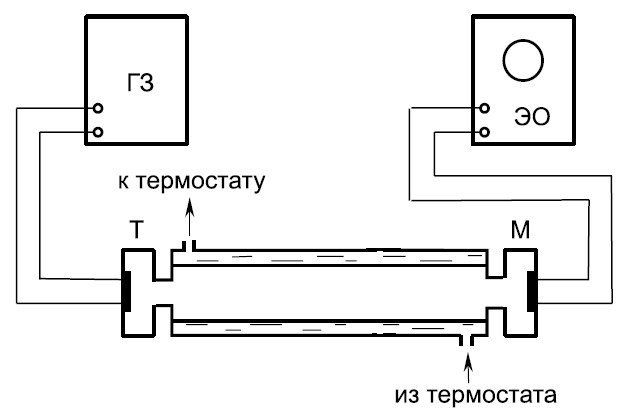
\includegraphics[width=12cm]{ust2.jpg}
	\end{center}
	\caption{\textit{Установка для изучения зависимости скорости звука от температуры}}
	\label{img2}
\end{figure}
% \begin{figure}[h!]
% 	\begin{center}
% 		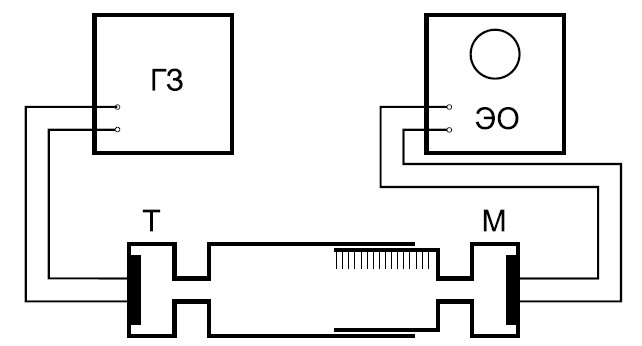
\includegraphics[width=12cm]{ust1.jpg}
% 	\end{center}
% 	\caption{\textit{Установка для измерения скорости звука при помощи раздвижной трубы}}
% 	\label{img1}
% \end{figure}

\newpage


\section*{Обработка данных}

Проведём измерения $ C_p/C_v $ для воздуха при различных температурах. Для этого будем использовать трубу постоянного размера $ L = (700 \pm 1) $ мм. Для фиксированной температуры будем изменять частоту звукового сигнала, тем самым изменяя и длину волны, так, чтобы мы могли наблюдать последовательные резонансы. Для каждого резонанса будем фиксировать частоту, при которой он возник. Полученные измерения занесём в таблицу %\ref{tab:constL}.

\begin{table}[h!]
	\centering
	\begin{tabular}{|lllll|}
		\hline
		\multicolumn{1}{|c|}{}    & \multicolumn{4}{|c|}{Температура, C}                                                                \\ \cline{2-5}
		\multicolumn{1}{|c|}{$n$} & \multicolumn{1}{l|}{22.4}            & \multicolumn{1}{l|}{32.1} & \multicolumn{1}{l|}{43.9} & 52.0 \\ \cline{2-5}
		\multicolumn{1}{|c|}{}    & \multicolumn{4}{c|}{$\nu$, Гц}                                                                      \\ \hline
		\multicolumn{1}{|l|}{1}   & \multicolumn{1}{l|}{255}             & \multicolumn{1}{l|}{257}  & \multicolumn{1}{l|}{265}  & 270  \\ \hline
		\multicolumn{1}{|l|}{2}   & \multicolumn{1}{l|}{497}             & \multicolumn{1}{l|}{505}  & \multicolumn{1}{l|}{511}  & 523  \\ \hline
		\multicolumn{1}{|l|}{3}   & \multicolumn{1}{l|}{739}             & \multicolumn{1}{l|}{747}  & \multicolumn{1}{l|}{760}  & 775  \\ \hline
		\multicolumn{1}{|l|}{4}   & \multicolumn{1}{l|}{990}             & \multicolumn{1}{l|}{1003} & \multicolumn{1}{l|}{1017} & 1026 \\ \hline
		\multicolumn{1}{|l|}{5}   & \multicolumn{1}{l|}{1231}            & \multicolumn{1}{l|}{1259} & \multicolumn{1}{l|}{1273} & 1285 \\ \hline
	\end{tabular}
	\caption{Результаты экспериментов}
\end{table}

%Также занесём в таблицу величину $ f_k = \hat{f_k} - \hat{f_0} $. Погрешность измерения такой величины составит $ \sigma_{f_k} = \sigma_{\hat{f_k}}\sqrt{2} \approx 2,82 $ Гц.

По полученным экспериментальным данным построим графики зависимости $ f_n(n) $.

\begin{figure}[h!]
	\subcaptionbox*{22.4 C}[.5\linewidth]{%
		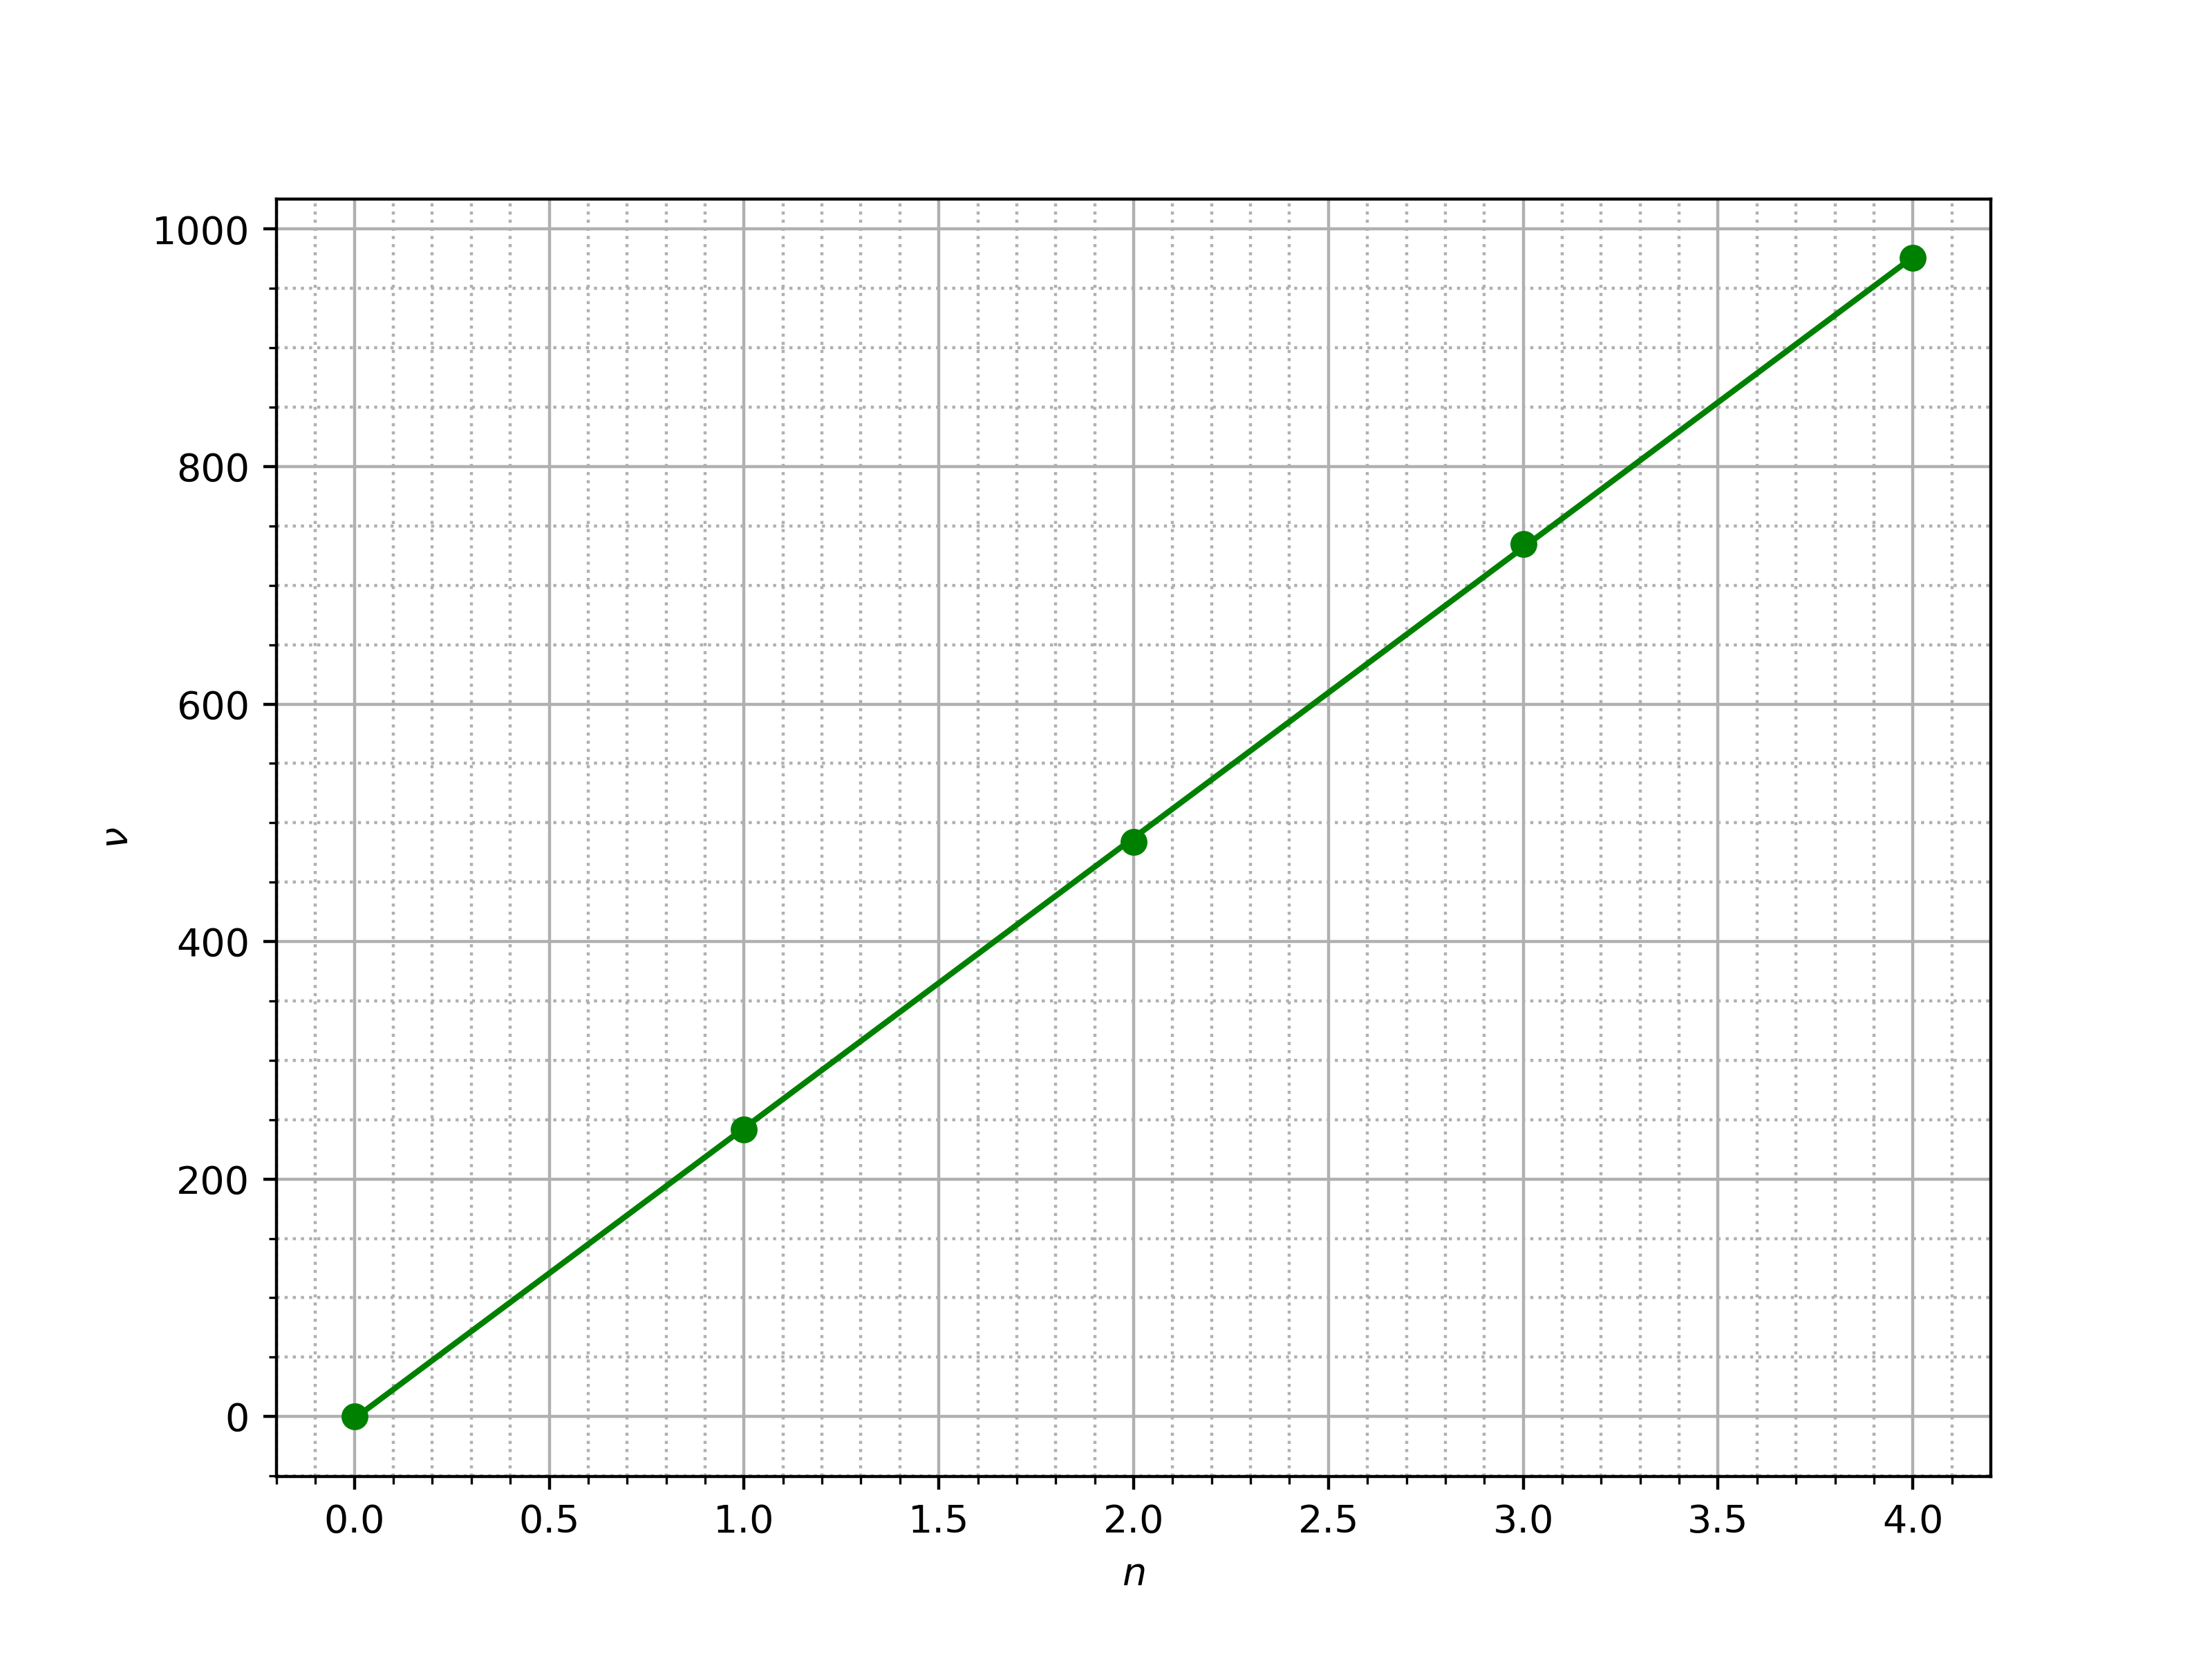
\includegraphics[width=\linewidth]{first.png}%
	}%
	\hfill
	\subcaptionbox*{32.1 C}[.5\linewidth]{%
		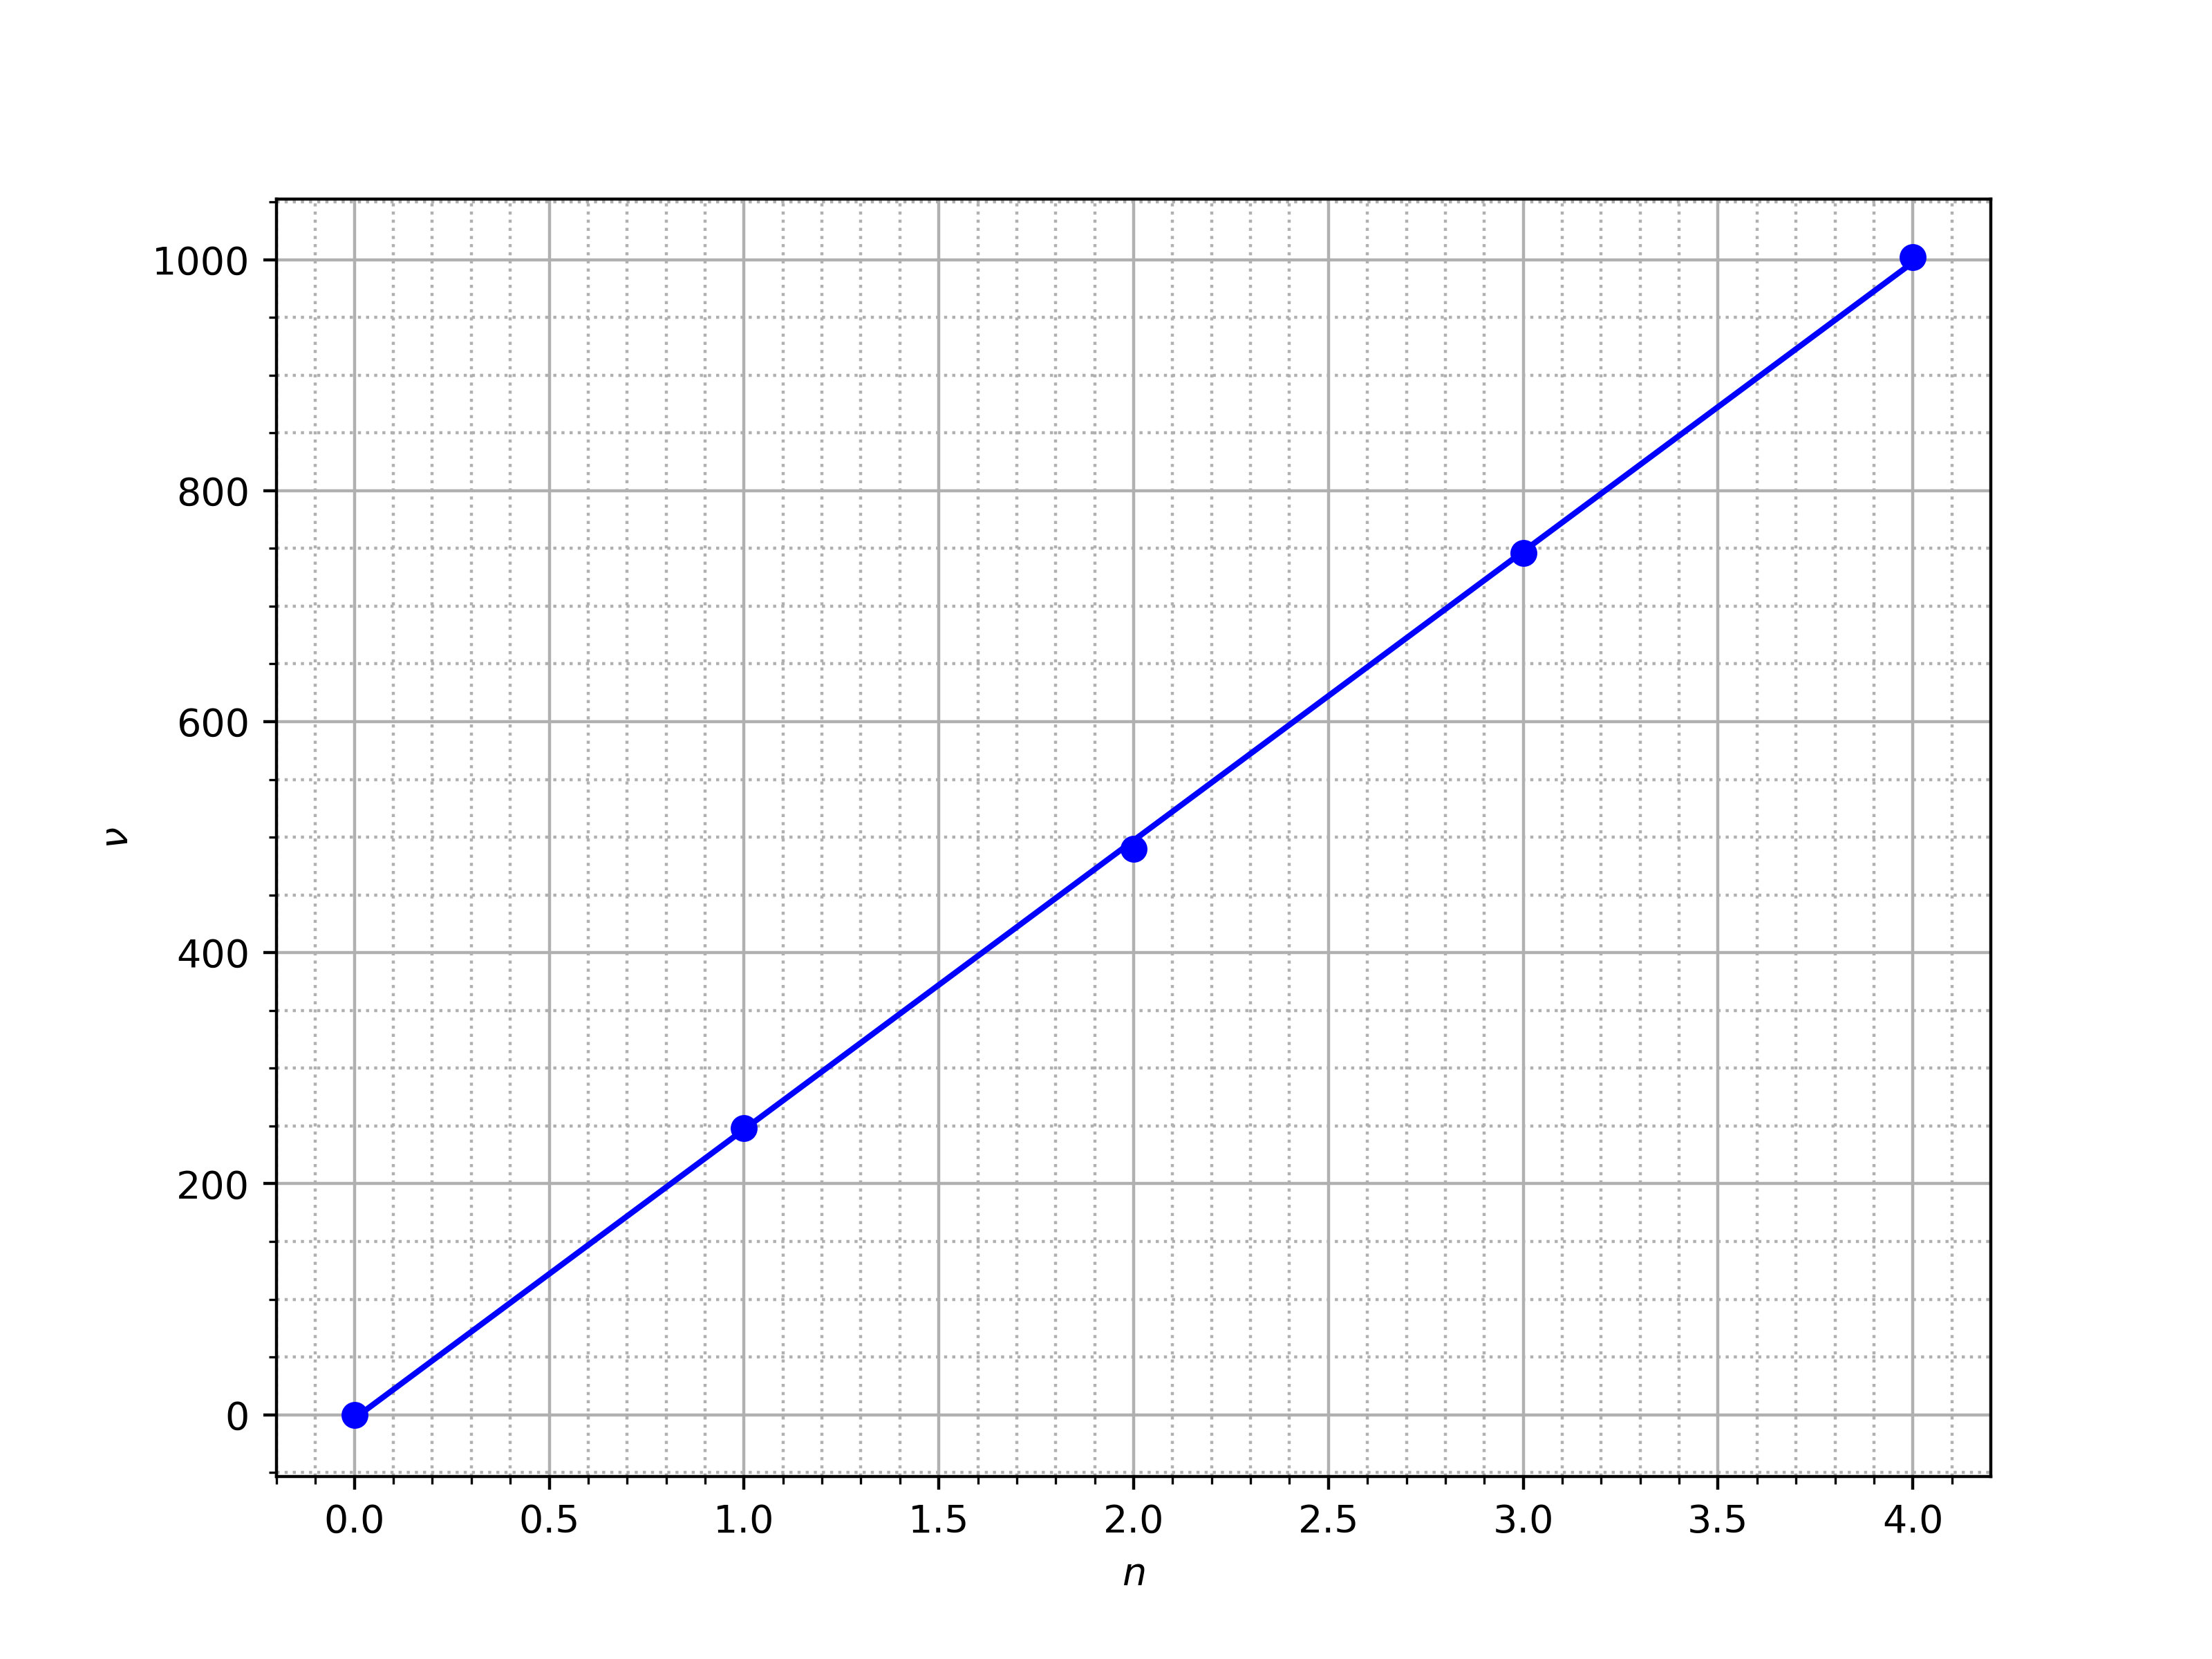
\includegraphics[width=\linewidth]{second.png}%
	}
	\subcaptionbox*{43.9 C}[.5\linewidth]{%
		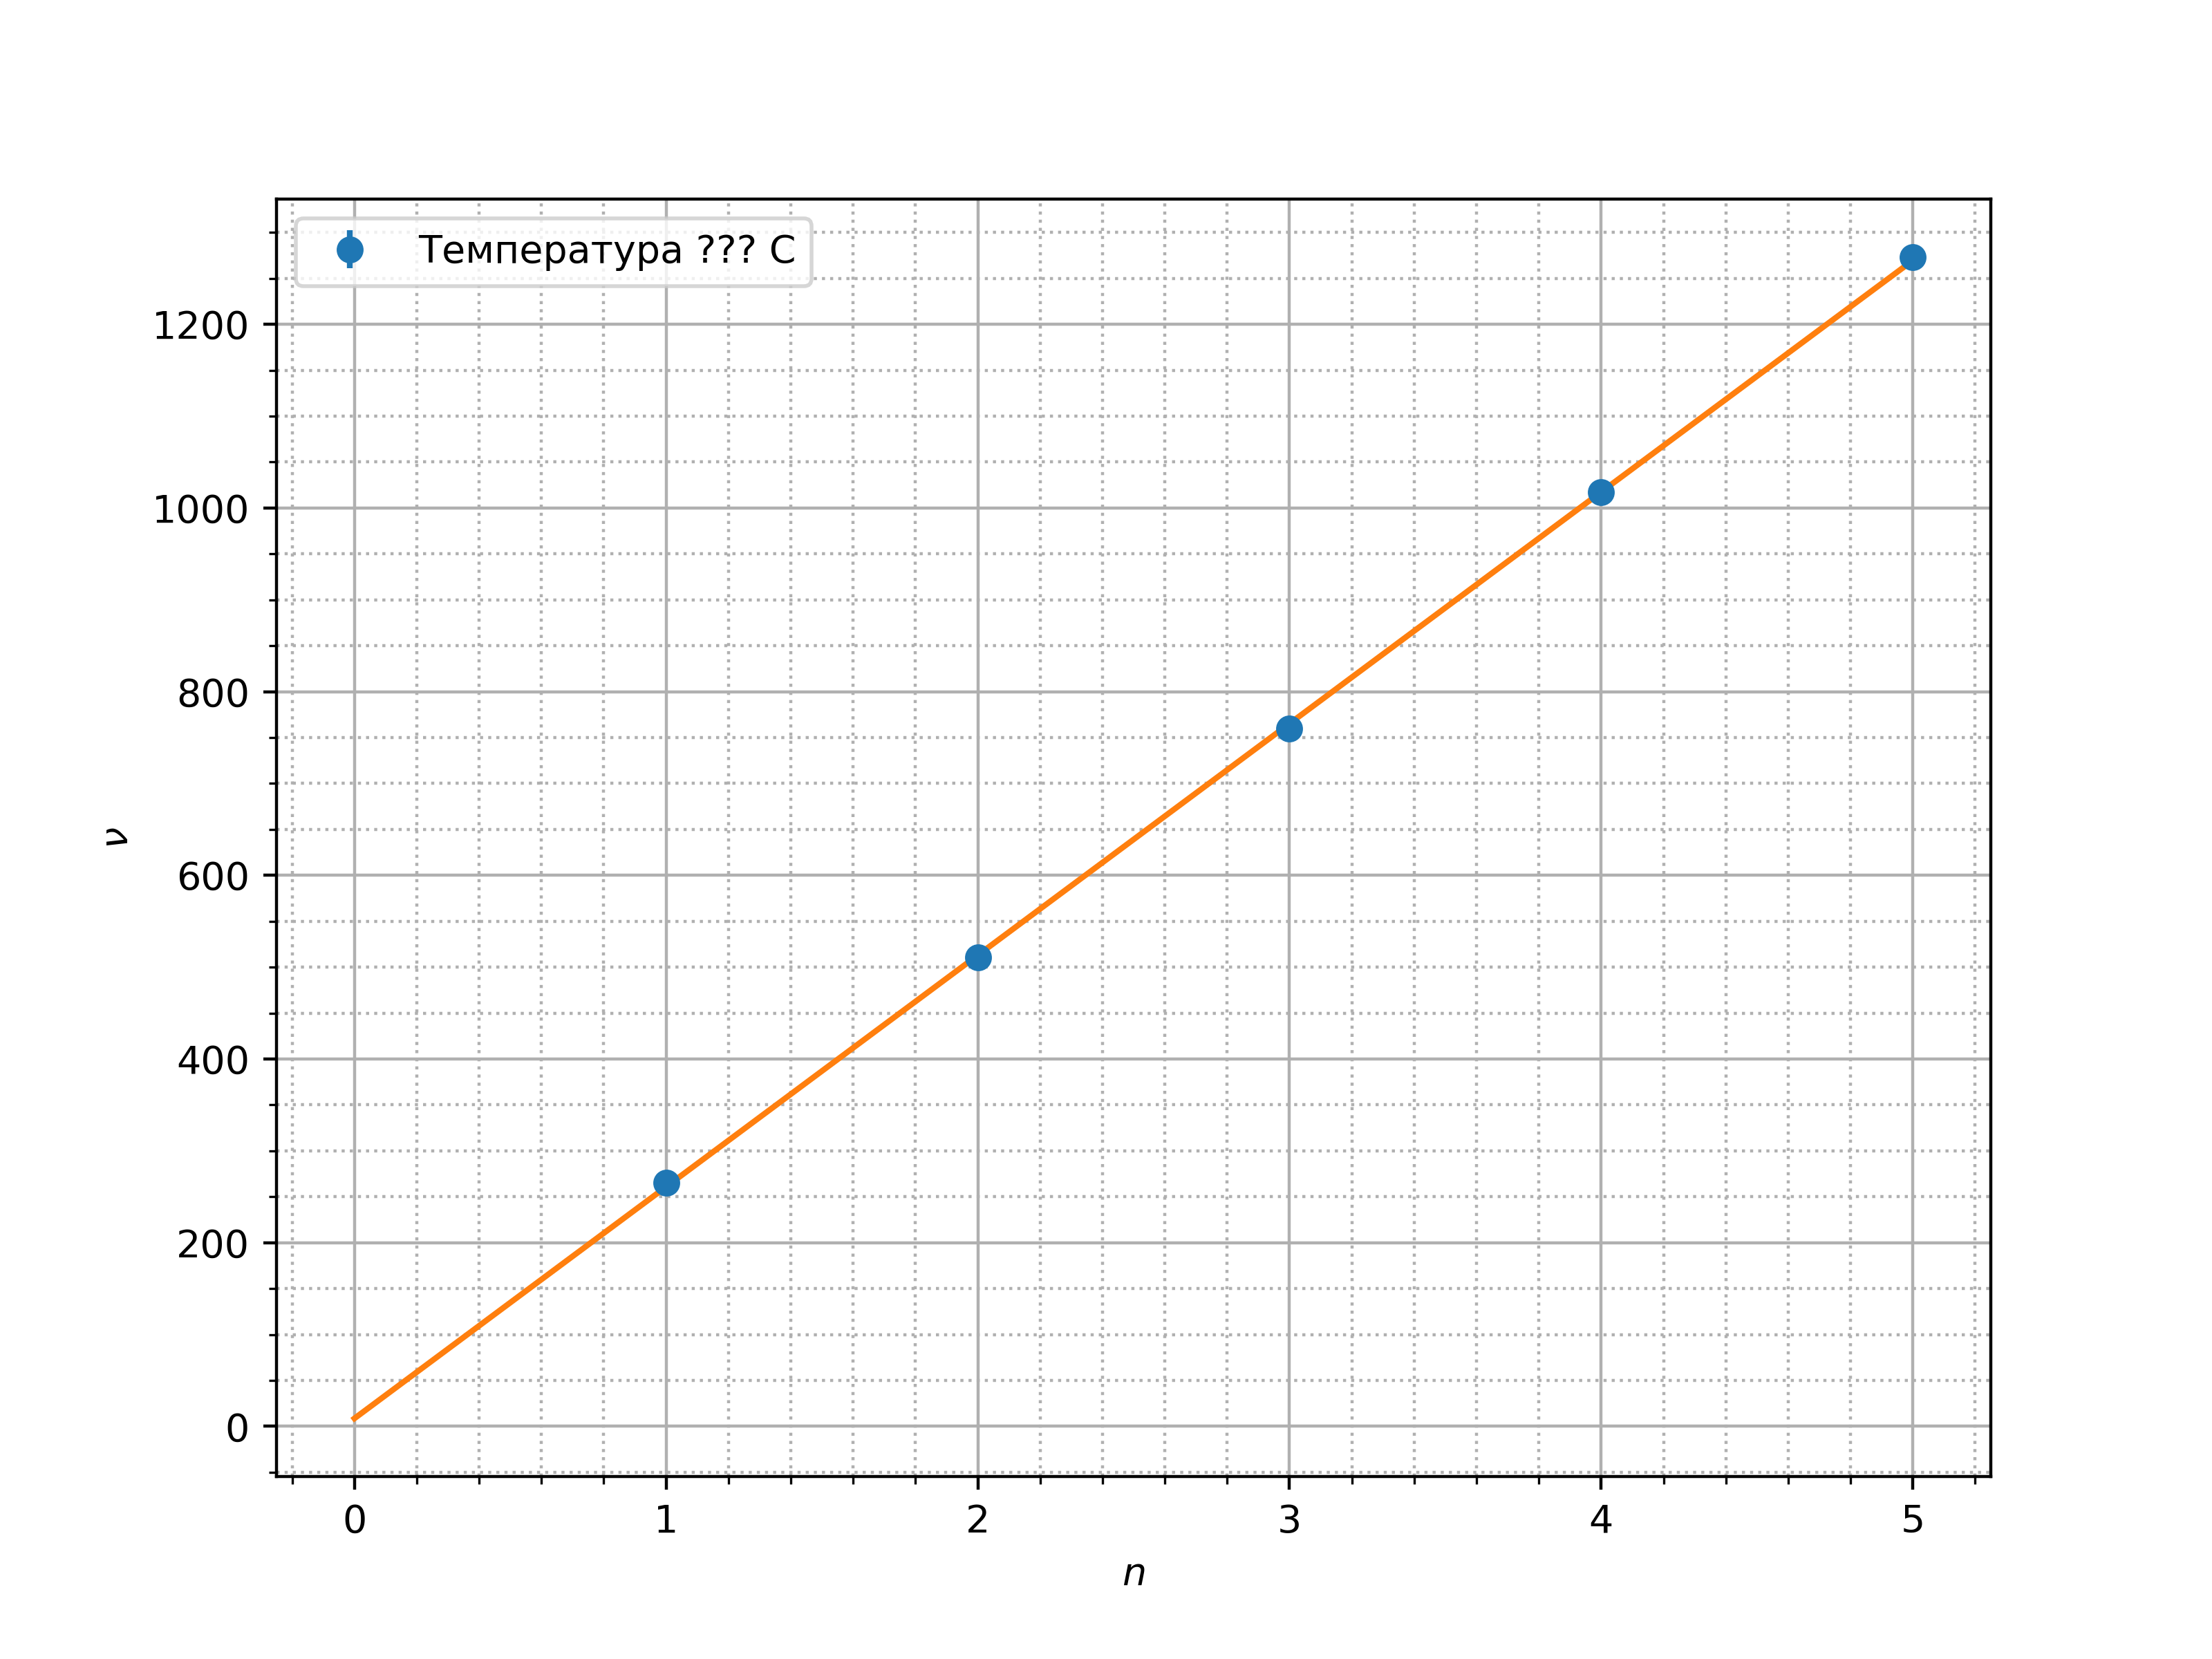
\includegraphics[width=\linewidth]{third.png}%
	}%
	\hfill
	\subcaptionbox*{52.0 C}[.5\linewidth]{%
		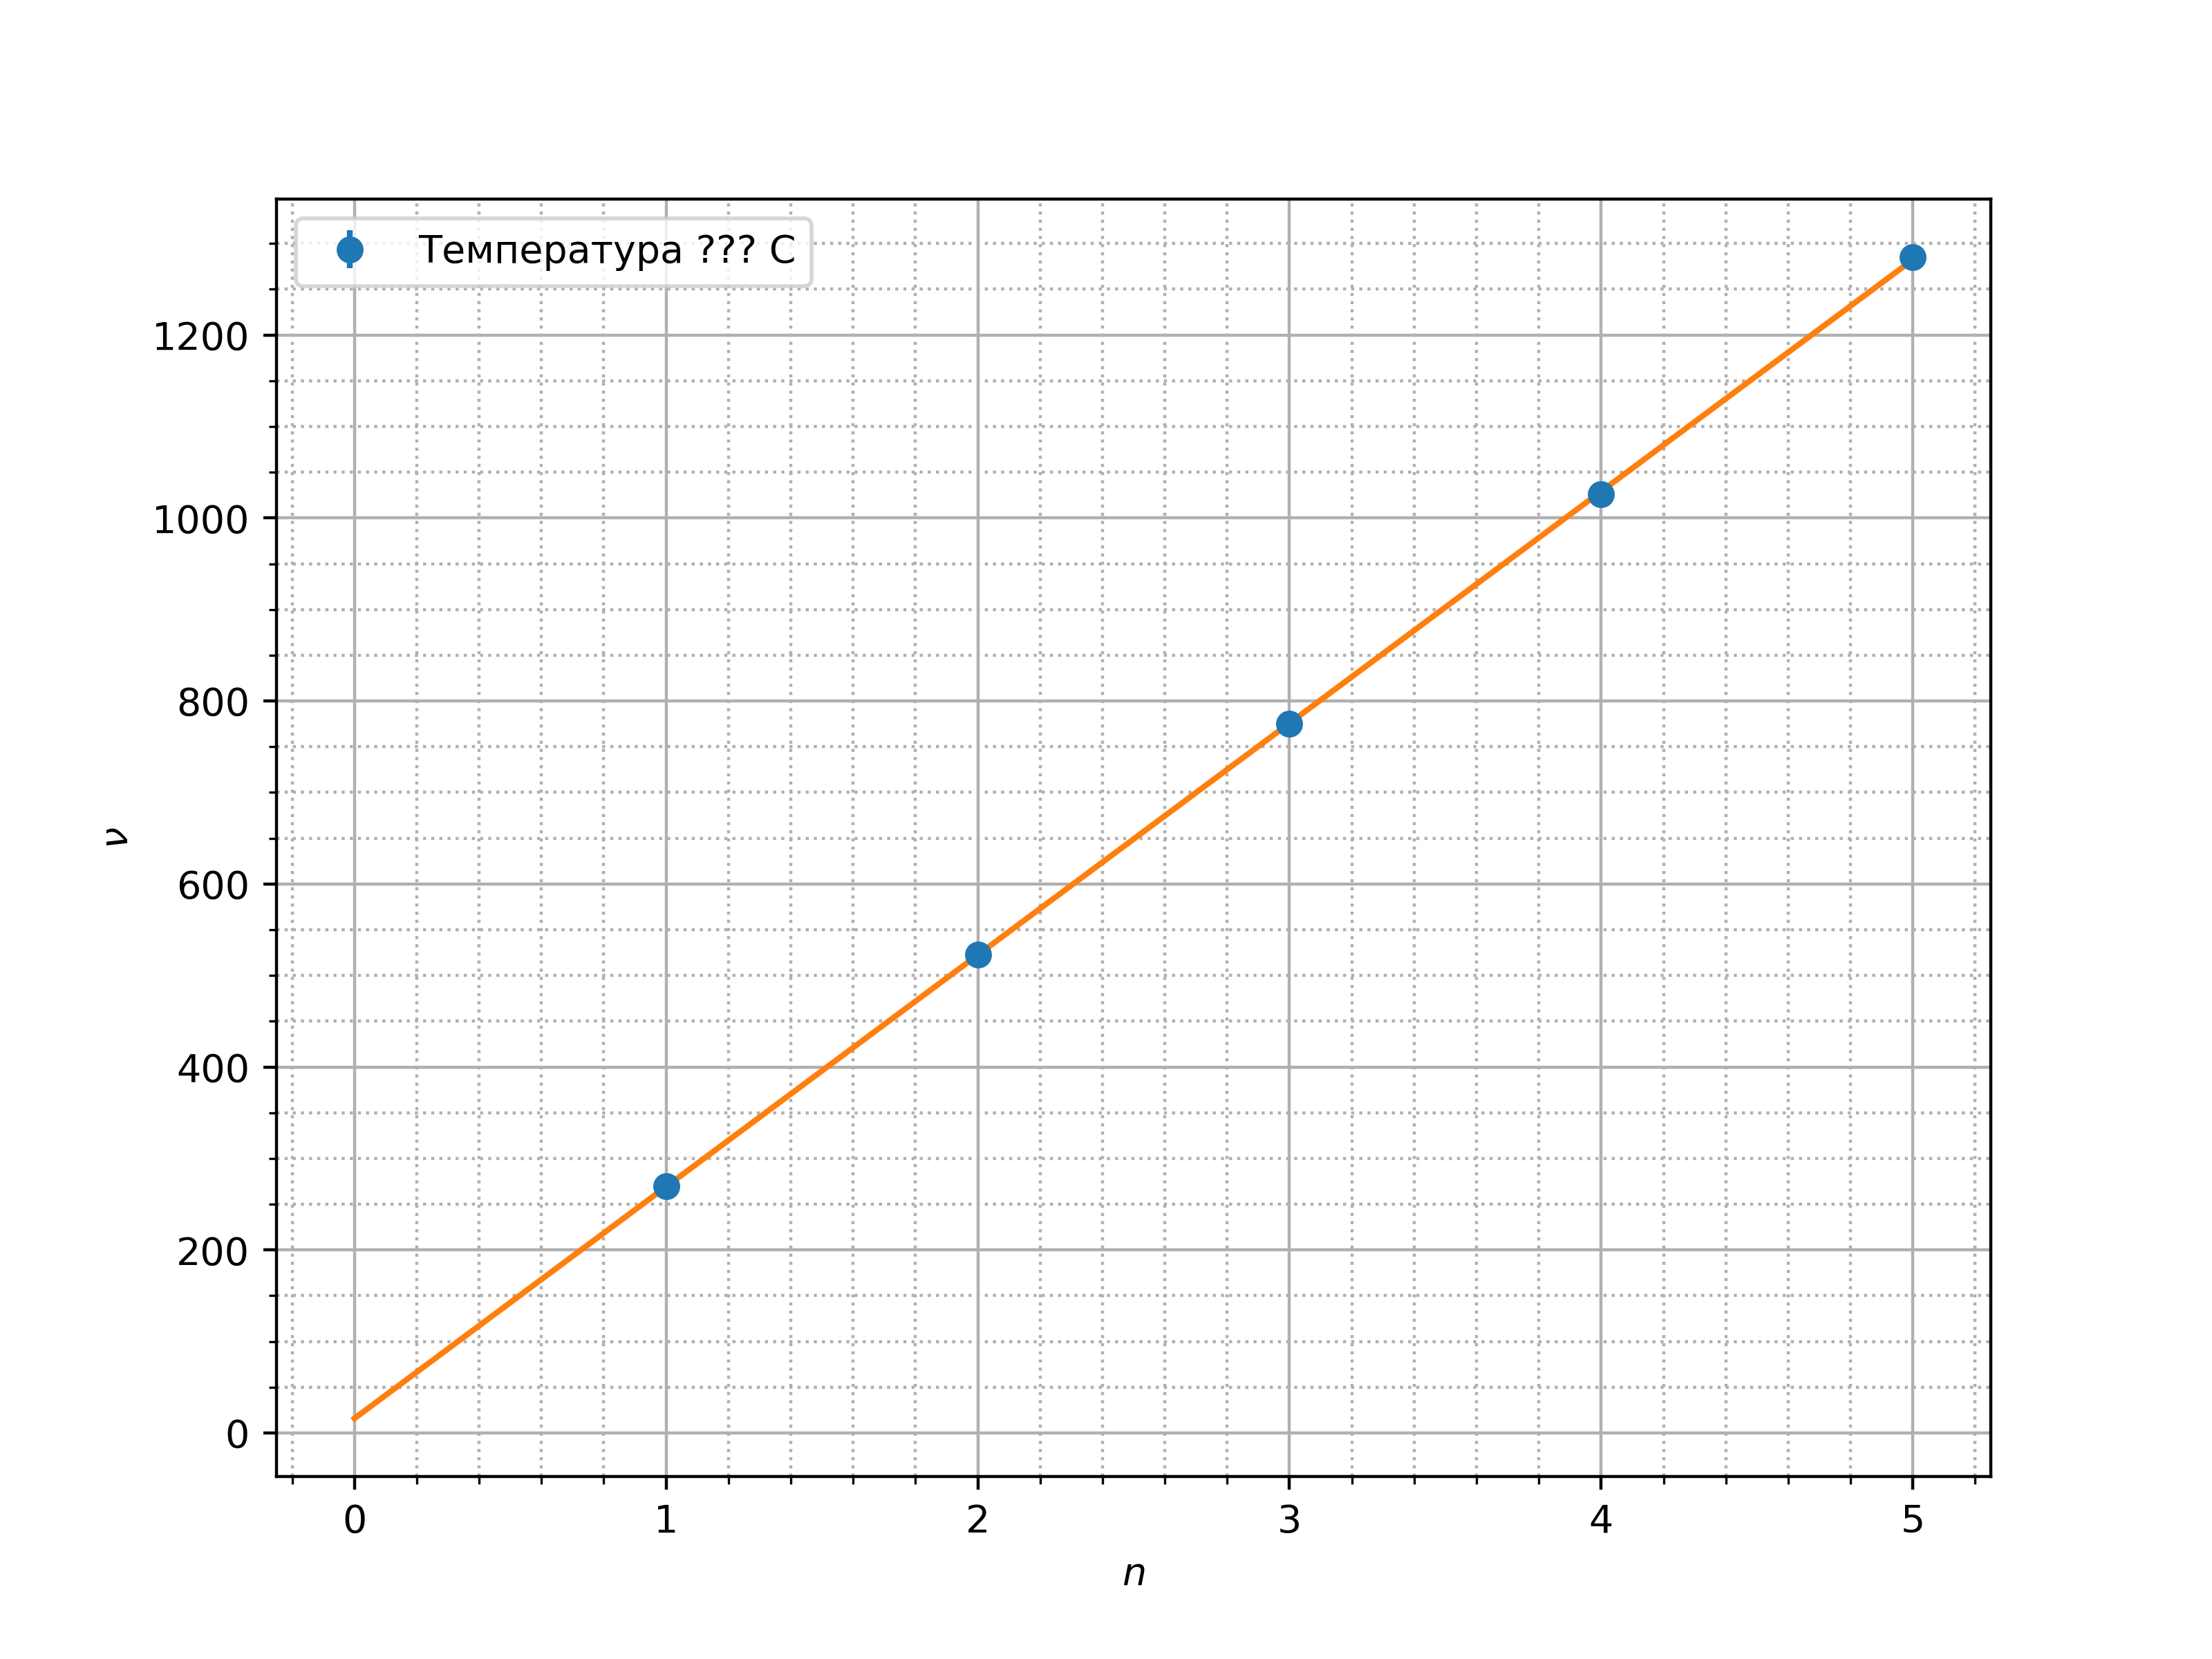
\includegraphics[width=\linewidth]{fourth.png}%
	}
	\caption{Экспериментально полученные точки и аппроксимации}
\end{figure}

\newpage

\begin{figure}[h!]
	\centering
	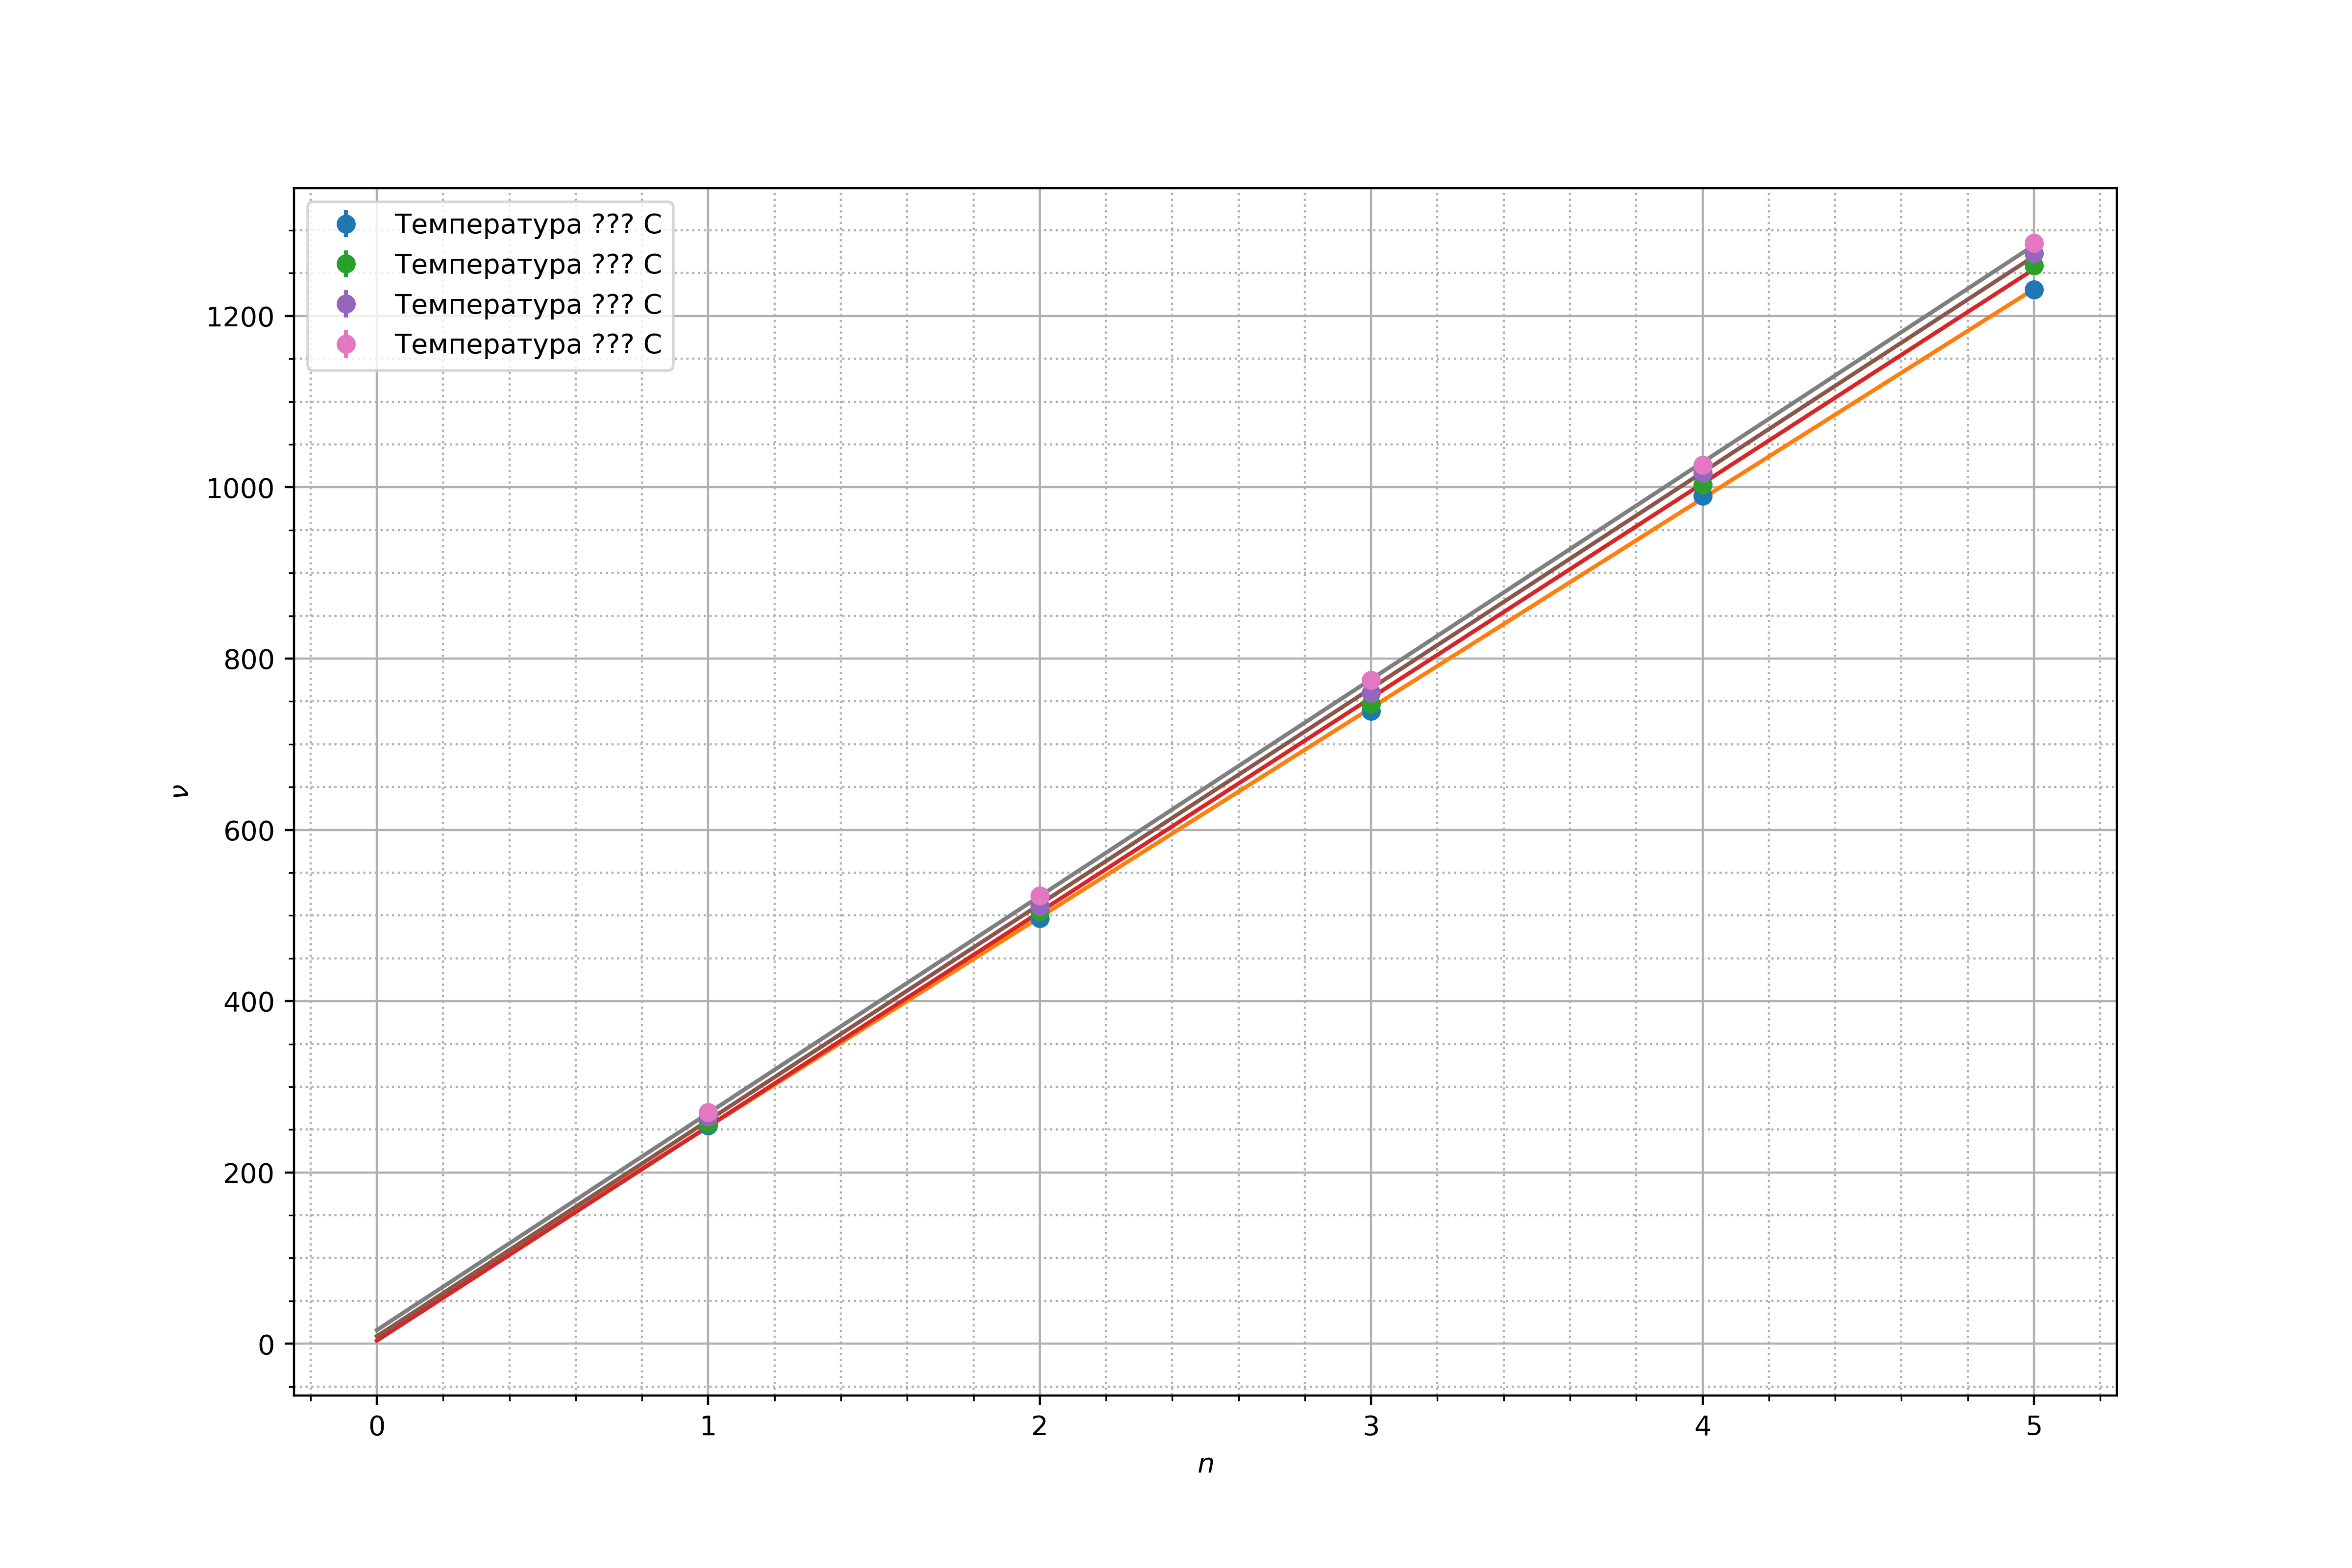
\includegraphics[width=0.7\textwidth]{all_in_one.png}
	\caption{Экспериментально полученные точки и аппроксимации}
\end{figure}

Аппроксимируем полученные зависимости прямыми $ y=kx $ используя метод наименьших квадратов. $k$ и их погрешности рассчитываем с помощью \texttt{numpy}. Результаты заносим в таблицу \ref{tab:resConstL}

Cогласно формуле \eqref{5}:
$$k = \frac{c}{2L} \Rightarrow c = 2 L k$$
$$\sigma_c = c\sqrt{\varepsilon_L^2 + \varepsilon_k^2}$$

\begin{table}[h!]
	\centering
	\begin{tabular}{|c|c|c|}
		\hline
		$ T $, $^{\circ}C$ & $\varepsilon_L$ & $\varepsilon_k$ \\ \hline
		22.4               & 0.001           & 0.003           \\ \hline
		32.1               & 0.001           & 0.005           \\ \hline
		43.9               & 0.001           & 0.004           \\ \hline
		52.0               & 0.001           & 0.002           \\ \hline
	\end{tabular}
\end{table}

\noindent Рассчитываем $c$ и его погрешность. Результаты заносим в таблицу \ref{tab:resConstL}.

Кроме того, по формуле \eqref{gamma}:

$$\gamma = \frac{\mu}{RT}c^2$$
$$\sigma_\gamma = \gamma\sqrt{\varepsilon_T^2+ 2\varepsilon_c^2}$$
\begin{table}[h!]
	\centering
	\begin{tabular}{|c|c|c|}
		\hline
		$ T $, $^{\circ}C$ & $\varepsilon_T$ & $\varepsilon_c$ \\ \hline
		22.4               & 0.0002          & 0.0032          \\ \hline
		32.1               & 0.0002          & 0.0054          \\ \hline
		43.9               & 0.0002          & 0.0056          \\ \hline
		52.0               & 0.0002          & 0.0027          \\ \hline
	\end{tabular}
\end{table}

\noindent Рассчитываем $\gamma$ и его погрешность, заносим результаты в таблицу \ref{tab:resConstL}.

\begin{table}[h!]
	\centering
	\begin{tabular}{|c|c|c|c|c|c|c|}
		\hline
		$ T $, $^{\circ}C$ & $k$, с$^{-1} $ & $ \sigma_k $, с$^{-1} $ & $c$, м/с & $\sigma_c$, м/с & $\gamma$ & $\sigma_\gamma$ \\ \hline
		22.4               & 342.3          & 1.1                     & 342.3    & 1.1             & 1.384    & 0.005           \\ \hline
		32.1               & 350.3          & 1.2                     & 350.3    & 1.9             & 1.403    & 0.008           \\ \hline
		43.9               & 353.1          & 1.1                     & 353.1    & 1.6             & 1.373    & 0.006           \\ \hline
		52.0               & 354.6          & 0.6                     & 354.6    & 1.0             & 1.350    & 0.004           \\ \hline
	\end{tabular}
	\caption{Результаты вычислений при различных температурах}
	\label{tab:resConstL}
\end{table}

Согласно полученным данным, можно утверждать, что $ \gamma $ остаётся постоянной в исследуемом диапазоне температур. Поэтому усредним результаты, полученные при различных значениях температуры и получим для воздуха:

\[ \boxed{\gamma = 1.378 \pm 0.003}\quad (\varepsilon=0.2\%) \]

Сравним полученные данные с табличными. Согласно справочнику, показатель адиабаты для воздуха при нормальных условиях равен \underline{$ \gamma = 1,4 $}. Результаты измерения незначительно отличаются от табличных.

\section*{Обсуждение результатов}

В результате проделанной работы:

\begin{itemize}
\item определен показатель адиабаты с помощью уравнения зависимости скорости распространения звуковой волны в газах:

$ \gamma = 1.378 \pm 0.003\quad (\varepsilon=0.2\%) $
\item получена величина скорости звука в воздухе при разных температурах
\begin{itemize}
\item $ c = 342.3 \pm 1.1\quad (\varepsilon=0,3\%) $ при $ T = 22.4^{\circ}C $
\item $ c = 350.3 \pm 1.9\quad (\varepsilon=0,5\%) $ при $ T = 32.1^{\circ}C $
\item $ c = 353.1 \pm 1.6\quad (\varepsilon=0,5\%) $ при $ T = 43.9^{\circ}C $
\item $ c = 354.6 \pm 1.0\quad (\varepsilon=0,3\%) $ при $ T = 52.0^{\circ}C $
\end{itemize}

\end{itemize}

Результаты измерения незначительно отличаются от табличных. Это может быть связано с большой неточностью определения резонансных частот на второй установке. Чтобы этого избежать, необходимо использовать генератор частоты с возможностью более точной настройки для возможности чёткого отслеживания резонансов.

\section*{Выводы}

В ходе данной работы:

\begin{enumerate}

\item определен показатель адиабаты для воздуха при помощи установки, на которой длина трубы оставалась постоянной на протяжении всего опыта, а резонансы достигались при помощи изменения частоты звукового сигнала

\item исследована зависимость коэффициента адиабаты $ \gamma $ от температуры газа. Было получено, что показатель адиабаты не зависит от температуры в диапазоне температур $ 20-60 $ $ ^\circ C $

\[ \boxed{\gamma_L = 1.378 \pm 0.003}\quad (\varepsilon=0.2\%) \]

\item измерены частоты колебаний звуковых волн при резонансе в воздухе, заполняющем трубу.
\end{enumerate}
\end{document}